\documentclass[12pt,french]{article}
\input preambule_2013

\newcounter{exoc}
\newenvironment{exoc}[1]{%
  \refstepcounter{exoc}\textbf{Exercice \theexoc} :\hfill {\footnotesize\textbf{(#1)}}\par
  \medskip}%
{\medskip}

\pagestyle{fancy}
\pieddepage{}{\thepage}{}

\setlength{\textheight}{26cm}% Hauteur de la zone de texte

\begin{document}


\begin{center}
\begin{tabularx}{\textwidth}{|>\centering m{2.5cm}|>\centering X|>{\centering\arraybackslash} m{2.5cm}|}
	\hline
		1\iere \bsc{S.t.i.2d.} &  Lundi 7 avril \np{2014} & \textbf{Bilan annuel} \\
	\hline
		\multicolumn{3}{|c|}{\bsc{Contrôle de mathématiques}} \\
	\hline
        \multicolumn{1}{|r}{\bsc{Nom}:} & \multicolumn{2}{l|}{} \\
		\multicolumn{1}{|r}{Prénom:} & \multicolumn{2}{l|}{} \\
	\hline
        \multicolumn{3}{|l|}{\bfseries Note et observations :} \\[1cm]
    \hline
\end{tabularx}\bigskip

{\itshape
La calculatrice est \textbf{autorisée}. Les feuilles de brouillon personnelles sont \textbf{interdites}.\par
La qualité et la précision de la rédaction seront prises en compte dans l'appréciation des copies.\par
Le barème est indicatif.\par\medskip
\textbf{\bsc{Attention} !! Le sujet est à rendre avec la copie.}
}
\end{center}

%-------------------------------------------------------------------------
%        EXERCICE 1
%-------------------------------------------------------------------------

\begin{exoc}{10 points -- Métropole - La Réunion - 11 septembre 2012}
    Si $A$ et $B$ sont deux événements, on rappelle que \[p(A) + p(B) = p(A \cup B) + p(A \cap B).\]
    Au départ d'une randonnée, trois itinéraires différents sont proposés à un groupe de 48 randonneurs : un itinéraire pour débutant, un de difficulté moyenne et un de niveau élevé.\par
    Ce groupe est composé de 32 femmes et de 16 hommes.\par
    Concernant le choix de l'itinéraire :
     \setlength\parindent{6mm}
         \begin{itemize}
            \item[$\bullet~~$] 5 femmes et 2 hommes choisissent l'itinéraire de niveau débutant ;
            \item[$\bullet~~$] 25\,\% des randonneurs choisissent l'itinéraire de difficulté moyenne et parmi eux, il y a autant de femmes que d'hommes ;
            \item[$\bullet~~$] Les autres randonneurs choisissent l'itinéraire de niveau élevé.
        \end{itemize}
     \setlength\parindent{0mm}

    On choisit au hasard un randonneur (on suppose que tous les randonneurs ont la même chance d'être choisis) et on note :\par
        $F$ l'évènement \og le randonneur est une femme \fg{} ;\par
        $H$ l'évènement\og le randonneur est un homme \fg{} ;\par
        $D$ l'évènement\og le randonneur choisit l'itinéraire de niveau débutant \fg{} ;\par
        $E$ l'évènement\og le randonneur choisit l'itinéraire de niveau élevé \fg.\par\medskip

    Tous les résultats des différents calculs seront donnés sous la forme d'une fraction irréductible. On pourra utiliser un arbre ou un tableau.\par\medskip

    \begin{enumerate}
        \item Calculer la probabilité $p(F)$ de l'évènement $F$.
        \item Calculer la probabilité $p(E)$ de l'évènement $E$.
        \item Définir par une phrase l'évènement noté $H \cap E$ et calculer sa probabilité $p(H \cap E)$.
        \item Montrer que la probabilité de l'évènement \og le randonneur est une femme ou choisit l'itinéraire de niveau débutant \fg{} est $\dfrac{17}{24}$.
        \item Dans cette question, on choisit au hasard un randonneur parmi les hommes.\par Quelle est la probabilité qu'il ait choisi l'itinéraire de niveau élevé ?
        \item Commenter et critiquer éventuellement cette phrase : \og Le niveau des femmes de ce groupe est plus élevé que celui des hommes \fg.
    \end{enumerate}
\end{exoc}\[*\]\clearpage

%-------------------------------------------------------------------------
%        EXERCICE 2
%-------------------------------------------------------------------------

\begin{exoc}{8 + 7 = 15 points -- Métropole - La Réunion - 11 septembre 2012 + Antilles - Guyane - 20 juin 2012}

Les deux parties sont indépendantes et peuvent être traitées séparément.\medskip

%----------------------------------------------------------------------------
\textbf{Partie} \rond{A}\medskip
%-----------------------------------------------------------------------------

    On considère les fonctions $f$ et $g$ définie sur $\R$ par :
    \[f(x) = x^2 \qetq g(x) = (x - 1)^2 - 4.\]
    On note $\calig C_f$ la courbe représentative de $f$ dans un repère orthogonal et $\calig C_g$ celle de $g$ dans le même repère.
    \begin{enumerate}
        \item Par quelle transformation géométrique passe-t-on de $\calig C_f$ à $\calig C_g$ ?
        \item Déterminer les coordonnées du sommet de $\calig C_g$.
        \item Dresser le tableau de variations de la fonction $g$.
        \item Dresser le tableau de signe de la fonction $g$ sur $\R$.
        \item Compléter directement sur le sujet le tableau de valeur suivant :
        \begin{center}
            \begin{tabular}{*{8}{|>{\centering\arraybackslash}m{1cm}}|}
                \hline
                    $x$ & $-3$ & $-2$ & $-1$ & $0$ & $1$ & $2$ & $3$ \\
                \hline
                    $g(x)$ & & & & & & & \\
                \hline
            \end{tabular}
        \end{center}
        \item Sur la page Annexe (page \pageref{Annexe}), on a représenté $\calig C_f$ dans un repère.\par Sur ce même repère, tracer précisément $\calig C_g$.
    \end{enumerate}\medskip

%----------------------------------------------------------------------------
\textbf{Partie} \rond{B}\medskip
%----------------------------------------------------------------------------

\begin{minipage}{0.5\linewidth}
    La parabole $\calig P$ ci-contre est la représentation graphique de la fonction polynôme $t$ définie sur l'ensemble $\R$ des nombres réels par :
    \[t(x) = ax^2 + bx + c\] où $a$, $b$ et $c$ désignent trois nombres réels que l'on se propose de déterminer dans cette partie.\par\medskip
\end{minipage}\hfill
\begin{minipage}{0.5\linewidth}
\begin{center}
    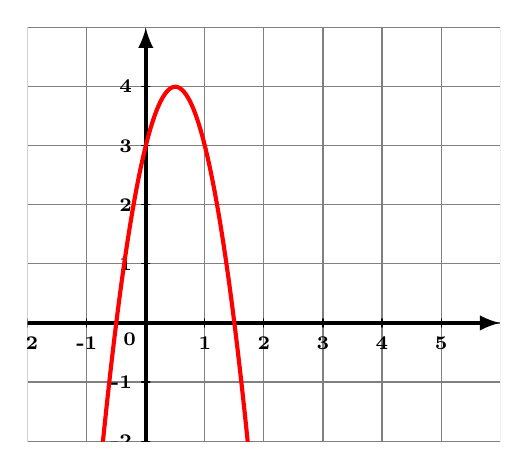
\begin{tikzpicture}[scale=0.75,line cap=round,line join=round,>=latex]
        \clip (-2,-2) rectangle (6,5);
        \draw[gray] (-2,-2) grid (6,5);
        \draw[->,line width=1.5pt] (-2,0)--(6,0);
        \draw[->,line width=1.5pt] (0,-2)--(0,5);
        \foreach \times in {-2,-1}
        \draw (\times,2pt) -- (\times,-2pt) node[below,font=\bfseries] {\scriptsize\times};
        \foreach \times in {1,...,5}
        \draw (\times,2pt) -- (\times,-2pt) node[below,font=\bfseries] {\scriptsize\times};
        \foreach \y in {1,...,4}
        \draw[color=black] (2pt,\y) -- (-2pt,\y) node[left,font=\bfseries] {\scriptsize\y};
        \foreach \y in {-2,-1}
        \draw[color=black] (2pt,\y) -- (-2pt,\y) node[left,font=\bfseries] {\scriptsize\y};
        \draw (0,0) node [below left,font=\bfseries] {\scriptsize 0};
        \draw [smooth,samples=200,domain=-3.5:3.5,line width=1.5pt,color=red] plot(\x,{-4*(\x)^2 + 4*\x + 3});
       % \draw [smooth,samples=200,domain=-3.5:3.5,line width=1.5pt,color=blue] plot(\x,{(\x - 1)^2-4});
    \end{tikzpicture}
\end{center}
\end{minipage}

\begin{enumerate}
    \item Démontrer à l'aide d'un calcul que $c = 3$.
    \item On sait que le point $S\left(\dfrac 12\pv 4\right)$ est le sommet de la parabole $\calig P$.\par
    En utilisant l'abscisse de $S$, démontrer que $a + b = 0$.
    \item En utilisant le fait que $t\left(\frac 1 2\right) = 4$, démontrer que $a + 2b = 4$.
    \item À l'aide des deux égalités précédentes, démontrer que $t(x) = -4x^2 + 4x + 3$.
    \item Déterminer les racines du polynôme $t$.
\end{enumerate}
\end{exoc}\[*\]\clearpage

%-------------------------------------------------------------------------
%        EXERCICE 3
%-------------------------------------------------------------------------

\begin{exoc}{7 + 8 = 15 points -- Antilles - Guyane - 19 juin 2013}
    Le plan complexe est rapporté à un repère orthonormé direct \Ouv (voir Annexe page \pageref{Annexe}).\par
    On note $\C$ l'ensemble des nombres complexes et on note $\ii$ le nombre complexe de module $1$ et d'argument $\dfrac \pi 2$.\par
    On rappelle que $\sqrt 8 = 2\sqrt 2$ et que $\dfrac{1}{\sqrt 2} = \dfrac{\sqrt 2}{2}$.\medskip

Les deux parties sont indépendantes et peuvent être traitées séparément.\medskip

%----------------------------------------------------------------------------
\textbf{Partie} \rond{A}\medskip
%-----------------------------------------------------------------------------

    On considère l'équation $(E)$ d'inconnue $z$ : \[(2 - \ii)z = 2 - 6\ii.\]
        \begin{enumerate}
            \item On appelle $z_1$ la solution de $(E)$ dans $\calig \C$. Démontrer que $z_1 = 2 - 2\ii$.
            \item Déterminer la forme trigonométrique de $z_1$.
            \item Soit $z_2 = -\ii \times z_1$.\par
            Déterminer la forme algébrique puis la forme trigonométrique de $z_2$.
        \end{enumerate}\medskip

%----------------------------------------------------------------------------
\textbf{Partie} \rond{B}\medskip
%-----------------------------------------------------------------------------

    Soit $A$, $B$ et $C$ les points du plan d'affixes respectives :
        \[z_A = 2 -2 \ii \qq z_B = -2 - 2\ii \qetq z_C = -4\ii.\]
            \begin{enumerate}
                \item Placer les points $A$, $B$ et $C$ dans le plan complexe de l'annexe page \pageref{Annexe}.
                \item Calculer les affixes $z_3$ et $z_4$ de $\vect{CA}$ et de $\vect{CB}$.
                \item Calculer le produit scalaire $\vect{CA}\cdot\vect{CB}$.
                \item Calculer $\norme{\vect{CA}}$ et $\norme{\vect{CB}}$.
                \item Déterminer la nature exacte du triangle $ABC$.
            \end{enumerate}
\end{exoc}\[*****\]

\clearpage

\begin{center}\label{Annexe}
    \Large\bfseries
    Annexe
\end{center}

\textbf{Exercice 2}\medskip

\begin{center}
    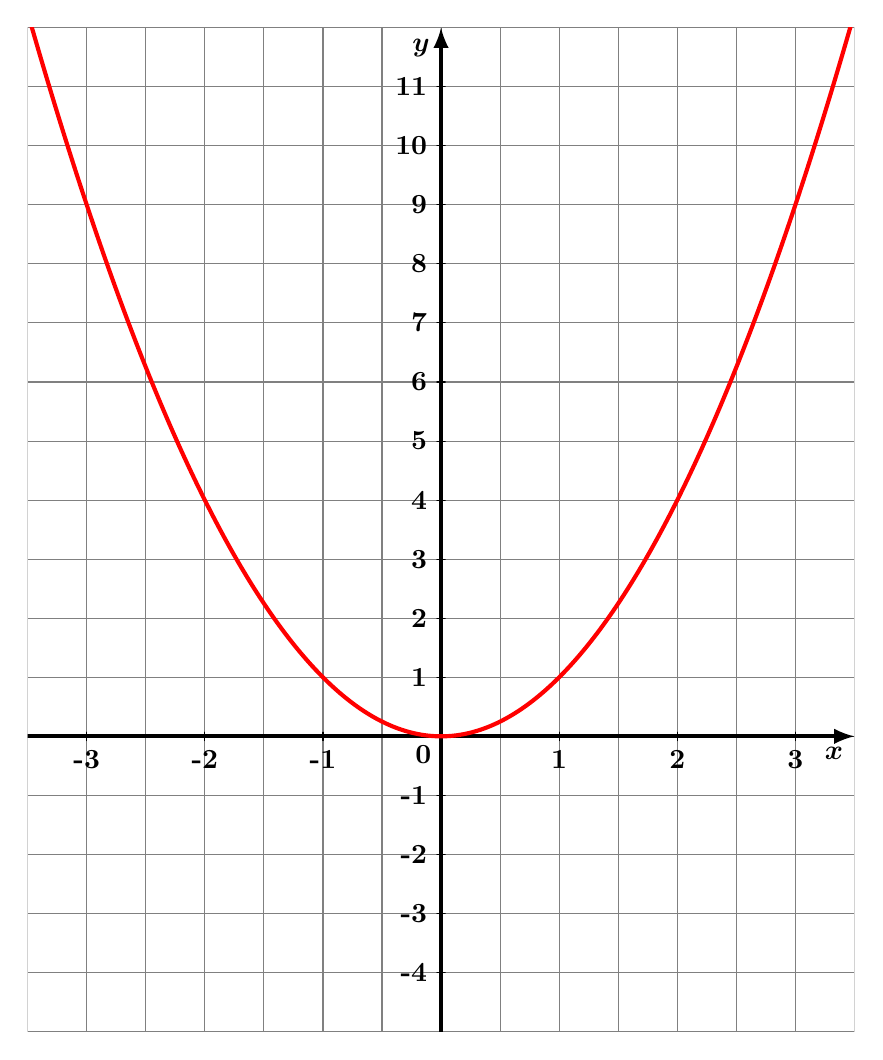
\begin{tikzpicture}[scale=0.75,line cap=round,line join=round,>=latex,x=2cm,y=1cm]
        \clip (-3.5,-5) rectangle (3.5,12);
        \draw[gray] (-3.5,-5)grid(3.5,12);
        \draw[->,line width=1.5pt] (-3.5,0)--(3.5,0)node[below left,font=\boldmath] {$x$};
        \draw[->,line width=1.5pt] (0,-5)--(0,12)node[below left,font=\boldmath] {$y$};
        \foreach \times in {-3,...,-1}
        \draw (\times,2pt) -- (\times,-2pt) node[below,font=\bfseries] {\times};
        \foreach \times in {1,...,3}
        \draw (\times,2pt) -- (\times,-2pt) node[below,font=\bfseries] {\times};
        \foreach \y in {1,...,11}
        \draw[color=black] (2pt,\y) -- (-2pt,\y) node[left,font=\bfseries] {\y};
        \foreach \y in {-4,...,-1}
        \draw[color=black] (2pt,\y) -- (-2pt,\y) node[left,font=\bfseries] {\y};
        \draw (0,0) node [below left,font=\bfseries] {0};
        \draw [smooth,samples=200,domain=-3.5:3.5,line width=1.5pt,color=red] plot(\x,{(\x)^2});
       % \draw [smooth,samples=200,domain=-3.5:3.5,line width=1.5pt,color=blue] plot(\x,{(\x - 1)^2-4});
    \end{tikzpicture}
\end{center}\[*\]

\textbf{Exercice 3}\medskip

\begin{center}
    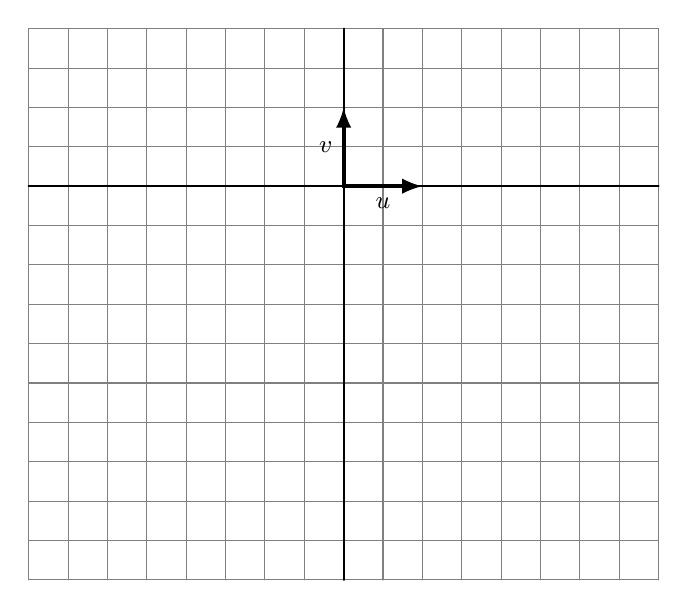
\begin{tikzpicture}[scale=0.5,line cap=round,line join=round,>=latex,x=2cm,y=2cm]
        \draw[gray] (-4,-5)grid(4,2);
        \draw[-,line width=0.75pt] (-4,0)--(4,0);
        \draw[-,line width=0.75pt] (0,-5)--(0,2);
        \draw[->, line width = 1.5pt] (0,0) -- (1,0) node[below,midway] {\small $\vect u$};
        \draw[->, line width = 1.5pt] (0,0) -- (0,1) node[left,midway] {\small $\vect v$};
    \end{tikzpicture}
\end{center}\[*****\]

\end{document} 